\section{Method}\label{sec:method}

%-------------------------------------------------------------------------------------------------------
\subsection{Network architecture}\label{subsec:architecture}
Since the dataset we use is lightweight, containing only 200,000 samples, it is essential to reuse pretrained weights from other network because training from scratch with small dataset would likely result in network overfitting and poor results on test data. As proposed in the paper, AlexNet is inherited in this project. However, this network only accepts inputs with three channels (e.g. RGB images), therefore it can only works with color images instead of depth maps. To bypass this issue, depth maps are colorized in the preprocessing step to convert the data from 1D to 3D. More information about this is discussed in Section \ref{subsec:preprocessing}.

Figure \ref{fig:architecture} illustrates the network's architecture, which can be broken into three networks: one for color-based classification, a network for depth-based classification, and one for fusion that combines the two single-modality streams into a final classification result. Architectures of single stream networks are inherited from AlexNet. However, the final fully connected layer (fc8) from the original network is only used for training single stream networks separately. To fuse them, that classification layer is replaced with two different ones: one for concatenating output from the two streams and one fully connected layer for classifying.

\begin{figure}
	\centering
    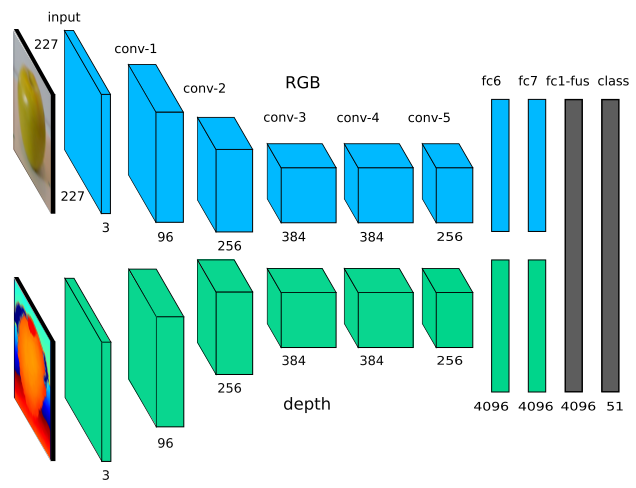
\includegraphics[width=\linewidth]{images/architecture}
    \caption{Fusion network architecture.}
    \label{fig:architecture}
\end{figure}

%-------------------------------------------------------------------------------------------------------
\subsection{Preprocessing}\label{subsec:preprocessing}
There are three primary steps in preprocessing: background removal, resizing, and depth colorization. The first step is straightforward as the mask for each sample is provided with the dataset. However, to test the effect of background removal, I also create another version of prepocessed data with background intact. 

For resizing, the images are rescaled to the shape of $256 \times 256$ although the network receives inputs of dimension $227 \times 227$. This is because we want to remove the mean image of original AlexNet, whose size is $256 \times 256$. After that, the images are randomly cropped to the size of $227 \times 227$ to produce jittering during training. To ensure the shape are not distorted, the images are scaled along the their longer side, the other side is padded with zero (color) and duplicated with boundary (depth), as showed in Figure \ref{fig:apple_3_viewpoints}. However, this does not affect if we remove background from the images.

The third step is to colorize depth. Depth sensors like the Xbox Kinect only give a single-channel intensity image proportional to the distance from the sensor. By converting depth images into three-channel data, we can treat them as images and feed into AlexNet (or other pretrained image recognition networks). Although there are different ways to colorize depth maps, jet colorization is proven superior in term of boosting system’s performance \cite{Eitel2015}.

%-------------------------------------------------------------------------------------------------------
\subsection{Network training}\label{sec:training}
The training process in divided into two different phases: (1) training the stream networks and (2) training the fusion network. Suppose that we have the dataset
\begin{equation}
	\mathcal{D} = \left\{ \left(\mathbf{x}^1, \mathbf{d}^1, \mathbf{y}^1\right), ..., \left(\mathbf{x}^N, \mathbf{d}^N, \mathbf{y}^N\right) \right\}
\end{equation}
where $\mathbf{x}^i$ is a RGB image, $\mathbf{d}^i$ is a depth image, and $\mathbf{y}^i$ is a label in the form of
\begin{align}
	\label{equ:label}
	\mathbf{y}^i &= (y_1^i, y_2^i, ..., y_k^i, ..., y_{M}^i)^\top \\
	\text{where} \qquad y_k^i &= 
	\begin{cases}
	1, & \mathbf{x}^i \text{ and } \mathbf{d}^i \text{ belong to class } k\\
	0, & \text{otherwise}
	\end{cases}
\end{align}
where $M$ is the number of classes. The data are fed into the first training phase and then the second one. In this project, I use Adam optimizer \cite{tensorflow2015-whitepaper}\cite{KingmaB14_adam}, included in TensorFlow, to minimize the loss. The learning rates are set as $10^{-3}$ for color and depth network and $10^{-5}$ for fusion; default decay rates of the optimizer is used.

\subsubsection{Training the stream networks}
Let $g^I(\mathbf{x}^i; \theta^I)$ be the representation for the color image $\mathbf{x}^i$ of the last fully connected layer from stream networks (\textit{fc7}) of AlexNet, where $\theta^I$ is the parameter. Similarly, we have $g^D(\mathbf{d}^i; \theta^D)$ for the depth image $\mathbf{d}^i$. Since we initialize the stream networks with pretrained weights, $\theta^I$ and $\theta^D$ are known. The weights $\mathbf{W}^I$ and $\mathbf{W}^D$ for RGB and depth streams are trained by solving
\begin{align}
	\min_{\mathbf{W}^I,\theta^I} &= \sum_{i=1}^N \mathcal{L} \left( \text{softmax}\left(\mathbf{W}^I g^I \left(\mathbf{x}^i; \theta^I\right), \mathbf{y}^i\right)\right), \\
	\min_{\mathbf{W}^D,\theta^D} &= \sum_{i=1}^N \mathcal{L} \left( \text{softmax}\left(\mathbf{W}^D g^D \left(\mathbf{d}^i; \theta^D\right), \mathbf{y}^i\right)\right),
\end{align}
where softmax function is
\begin{equation}
	\text{softmax}(z) =\frac{e^z}{\lVert z \rVert_1}
\end{equation}
and the loss is
\begin{equation}
	\mathcal{L}(x,y) = -\sum_k y_k \log s_k.
\end{equation}
This loss function is actually the ``categorical crossentropy'' function, which is commonly used in neural networks.

\subsubsection{Training the fusion network}
After acquiring $\mathbf{W}^I$ and $\mathbf{W}^D$, we discard the softmax layers (\textit{fc8}) and concatenate the last responses of the two streams: $g^I(\mathbf{x}^i; \theta^I)$ and $g^D(\mathbf{d}^i; \theta^D)$ and feed them through the additional fusion layer (\textit{fc1\_fus})
\begin{equation}
	\mathcal{F} = f\left(\left[g^I(\mathbf{x}^i; \theta^I); g^D(\mathbf{d}^i; \theta^D)\right]; \theta^F\right)
\end{equation}
where $\theta^F$ is the parameters of this layer. We can train this layer with a similar manner as in the previous training phase:
\begin{equation}
	\min_{\mathbf{W}^F,\theta^I, \theta^D, \theta^F} = \sum_{i=1}^N \mathcal{L} \left( \text{softmax}\left(\mathbf{W}^F \mathcal{F}, \mathbf{y}^i\right)\right)
\end{equation}

Note that in this phase, the weights trained from the previous one are kept unchanged as they play the role of feature extractor. Only the weights of the fusion network are optimized. 